\documentclass[11pt]{article}
\usepackage[english]{babel}
\usepackage{minted}
\usepackage{amsmath}
\usepackage{amsthm}
\usepackage{graphicx}
\usepackage{subcaption}
\usepackage{booktabs}
\usepackage{tikz}
\usepackage[left=25mm, top=25mm, bottom=30mm, right=25mm]{geometry}
\usepackage[colorlinks=true, linkcolor=blue, urlcolor=cyan, filecolor=magenta]{hyperref}

\usetikzlibrary{shapes.geometric, arrows}
\tikzstyle{startstop} = [rectangle, rounded corners, minimum width=3cm, minimum height=1cm,text centered, draw=black, fill=red!30]

\title{COL334\\Assignment 2}
\author{Sayam Sethi}
\date{September 2021}

\begin{document}

\maketitle

\tableofcontents

\section{Preliminaries}
The language used is \texttt{Java} since it offers cross-platform compatibility which is dubious in \texttt{C++} since there is no \textit{standard} library for socket programming. This might lead to incompatibility when running the code on a platform different from the one it has been implemented on. \texttt{Java} is better than \texttt{python} since \texttt{python} is a relatively slower language and networking applications need to be quick to deliver the best performance.

\section{\href{run:./Server.java}{Server.java}}
The logical flow of the server is given as follows:
\begin{center}
    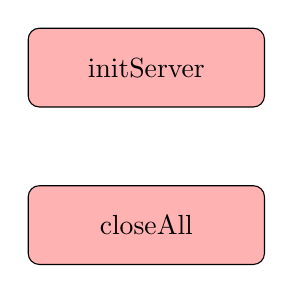
\begin{tikzpicture}[node distance=2cm]
        \node (start)[startstop]{initServer};
        \node (end)[startstop, below of=start]{closeAll};
    \end{tikzpicture}
\end{center}


\end{document}

